\documentclass{standalone}
\usepackage{tikz}
\usetikzlibrary{shapes.geometric}
\begin{document}

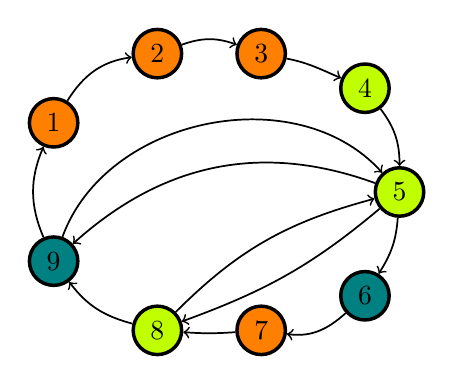
\begin{tikzpicture}
[every node/.style={inner sep=0pt}]
\node (3) [circle, minimum size=17.5pt, fill=orange, line width=1.25pt, draw=black] at (125.0pt, -25.0pt) {\textcolor{black}{3}};
\node (2) [circle, minimum size=17.5pt, fill=orange, line width=1.25pt, draw=black] at (87.5pt, -25.0pt) {\textcolor{black}{2}};
\node (1) [circle, minimum size=17.5pt, fill=orange, line width=1.25pt, draw=black] at (50.0pt, -50.0pt) {\textcolor{black}{1}};
\node (9) [circle, minimum size=17.5pt, fill=teal, line width=1.25pt, draw=black] at (50.0pt, -100.0pt) {\textcolor{black}{9}};
\node (4) [circle, minimum size=17.5pt, fill=lime, line width=1.25pt, draw=black] at (162.5pt, -37.5pt) {\textcolor{black}{4}};
\node (5) [circle, minimum size=17.5pt, fill=lime, line width=1.25pt, draw=black] at (175.0pt, -75.0pt) {\textcolor{black}{5}};
\node (8) [circle, minimum size=17.5pt, fill=lime, line width=1.25pt, draw=black] at (87.5pt, -125.0pt) {\textcolor{black}{8}};
\node (7) [circle, minimum size=17.5pt, fill=orange, line width=1.25pt, draw=black] at (125.0pt, -125.0pt) {\textcolor{black}{7}};
\node (6) [circle, minimum size=17.5pt, fill=teal, line width=1.25pt, draw=black] at (162.5pt, -112.5pt) {\textcolor{black}{6}};
\draw [line width=0.625, ->, color=black] (1) to  [in=188, out=58] (2);
\draw [line width=0.625, ->, color=black] (2) to  [in=160, out=20] (3);
\draw [line width=0.625, ->, color=black] (3) to  [in=157, out=349] (4);
\draw [line width=0.625, ->, color=black] (4) to  [in=90, out=307] (5);
\draw [line width=0.625, ->, color=black] (5) to  [in=58, out=266] (6);
\draw [line width=0.625, ->, color=black] (6) to  [in=352, out=222] (7);
\draw [line width=0.625, ->, color=black] (7) to  [in=356, out=184] (8);
\draw [line width=0.625, ->, color=black] (8) to  [in=307, out=165] (9);
\draw [line width=0.625, ->, color=black] (9) to  [in=247, out=113] (1);
\draw [line width=0.625, ->, color=black] (9) to  [in=132, out=70] (5);
\draw [line width=0.625, ->, color=black] (5) to  [in=42, out=160] (9);
\draw [line width=0.625, ->, color=black] (8) to  [in=195, out=45] (5);
\draw [line width=0.625, ->, color=black] (5) to  [in=20, out=220] (8);
\end{tikzpicture}

\end{document}
